\documentclass[a4paper,11pt]{article}
\usepackage[utf8]{inputenc}
\usepackage[italian]{babel}
\usepackage[margin=1.5cm,top=1cm,bottom=1cm]{geometry}
\usepackage{tikz,graphicx,amsmath,amssymb,booktabs,xcolor}
\usepackage{helvet}
\renewcommand{\familydefault}{\sfdefault}
\pagestyle{empty}
\begin{document}

\begin{minipage}[t][0.18\textheight]{\textwidth}
  \centering
  {\huge\bfseries (34713) Yesiltas occults GAIA 3441366322859801216}\\[0.3cm]
  {\LARGE\bfseries 2026-01-10 01:51:07 UT}\\[0.4cm]
  \begin{tabular}{p{0.31\textwidth} p{0.31\textwidth} p{0.31\textwidth}}
    \textbf{ASTEROIDE} & \textbf{STELLA} & \textbf{EVENTO} \\
    \midrule
    Diametro: 5.8 km & Mag: 14.1 & Calo mag: 2.6 \\
    Mag (H): 13.86 & RA: +85°56'59.91" & Durata max: 0.6 s \\
    P.U. Dist: 0 km & Dec: +26°30'43.70" & Incertezza: $\pm$0 km \\
  \end{tabular}
\end{minipage}
\vfill

\begin{minipage}[t][0.39\textheight]{\textwidth}
  \begin{minipage}[b]{0.49\textwidth}
    \centering
    {\bfseries Carta di Approccio (Visione d'Insieme)}\\[0.1cm]
    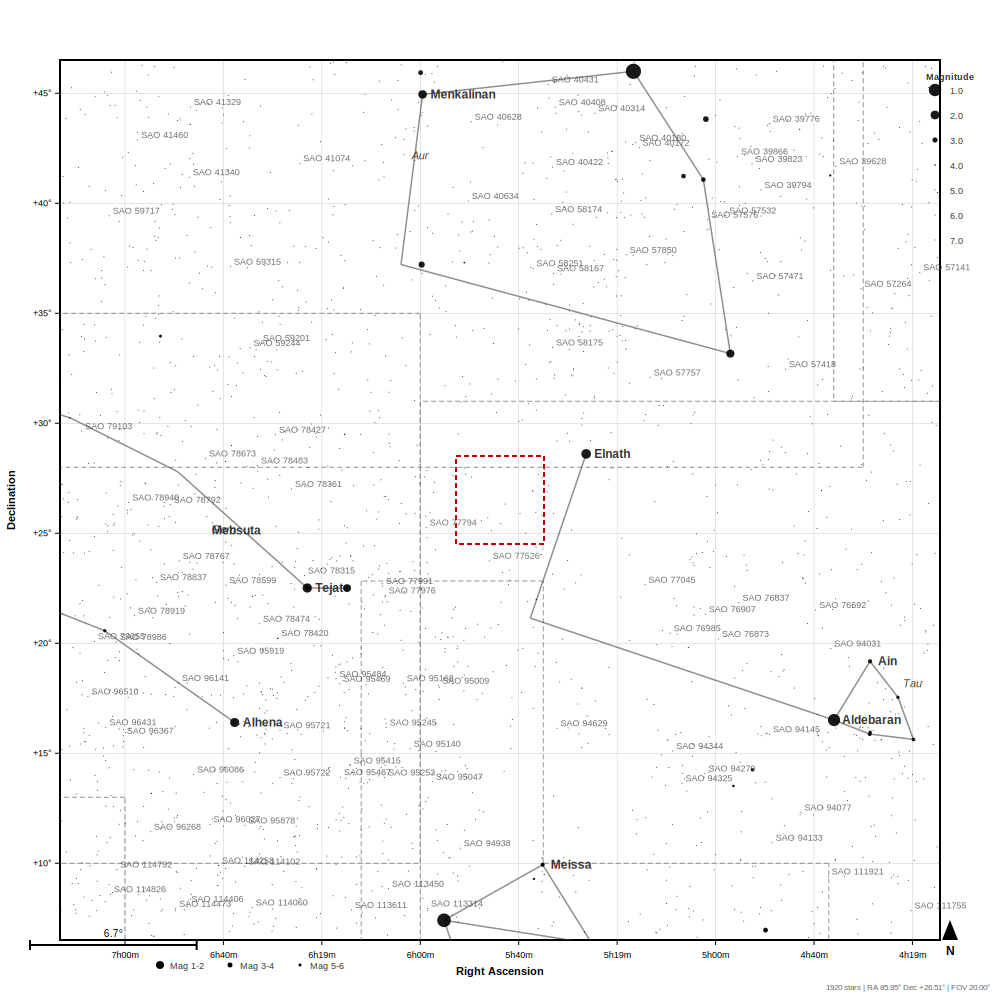
\includegraphics[width=\textwidth,height=0.35\textheight,keepaspectratio]{card_A4_34713_GAIA_DR3_3441366322859801216_approach.png}
  \end{minipage}
  \hfill
  \begin{minipage}[b]{0.49\textwidth}
    \centering
    {\bfseries Mappa dell'Occultazione al Suolo}\\[0.1cm]
    \includegraphics[width=\textwidth,height=0.35\textheight,keepaspectratio]{card_A4_34713_GAIA_DR3_3441366322859801216_earth.png}
  \end{minipage}
\end{minipage}
\vfill

\begin{minipage}[t][0.39\textheight]{\textwidth}
    \centering
    {\bfseries Carta di Lavoro (Finder - Campo Stretto)}\\[0.1cm]
    \includegraphics[width=\textwidth,height=0.35\textheight,keepaspectratio]{card_A4_34713_GAIA_DR3_3441366322859801216_finder.png}
\end{minipage}
\end{document}
